\documentclass{standalone}

\usepackage{tikz}

\usetikzlibrary{positioning, chains, shapes.geometric, fit, shapes, arrows.meta, calc, backgrounds}

\begin{document}

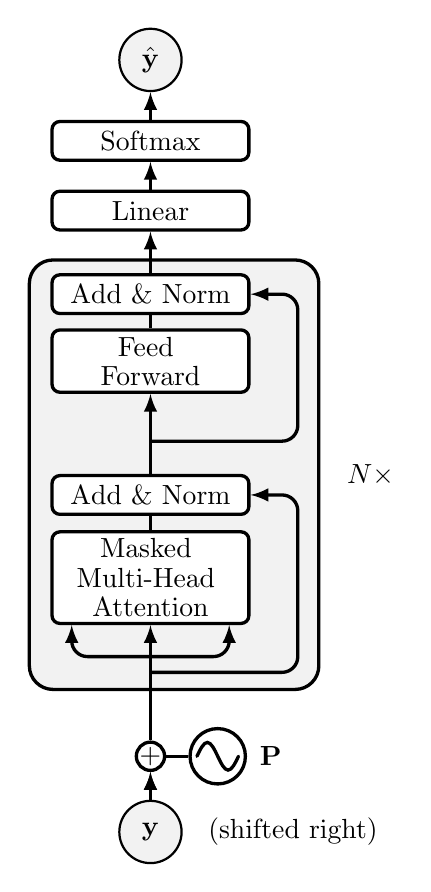
\begin{tikzpicture}[
    >=LaTeX, % Use default LaTeX arrows
    very thick,
    arrow/.style={
        -latex,
        very thick,
        rounded corners=0.2cm
    },
    block/.style={
        rectangle,
        fill=gray!10,
        rounded corners=3mm,
        draw,
        very thick
    },
    layer/.style={
        rectangle,
        fill=white!10,
        rounded corners=1mm,
        inner xsep=0em,
        inner ysep=0.25em,
        minimum height=1.4em,
        align=center,
        text width=2.5cm,
        draw,
        very thick
    },
    input/.style={ % Input or output node
        circle,
        minimum width=2.25em,
        draw,
        fill=gray!10,
        thick
    },
    do path picture/.style={%
        path picture={%
          \pgfpointdiff{\pgfpointanchor{path picture bounding box}{south west}}%
            {\pgfpointanchor{path picture bounding box}{north east}}%
          \pgfgetlastxy\x\y%
          \tikzset{x=\x/2,y=\y/2}%
          #1
        }
    },
    sin wave/.style={do path picture={    
        \draw [line cap=round] (-3/4,0)
        sin (-3/8,1/2) cos (0,0) sin (3/8,-1/2) cos (3/4,0);
        }
    }
]

    \node[input] (oemb) at (5.25,-0.45) {$\mathbf{y}$};

    % Sums
    \node[circle, draw, minimum size=0.25em, inner sep=0pt, above=1em of oemb] (sum2) {$\mathbf{+}$};
    % Positional Encoding
    \node [circle, draw, sin wave, minimum size=2em, right=0.8em of sum2] (pe2) {};

    % Decoder 1st sub-layer
    \node[layer] (add3) at (5.25,3.83) {Add \& Norm};
    \node[layer] (attn3) at (5.25,2.78) {Masked \vspace{-0.05cm} \linebreak Multi-Head \vspace{-0.05cm} \linebreak Attention};
    \draw[] (attn3) -- (add3);
    % Decoder 3rd sub-layer
    \node[layer] (add5) at (5.25,6.38) {Add \& Norm};
    \node[layer] (ff2) at (5.25,5.53) {Feed \vspace{-0.05cm} \linebreak Forward};
    \draw[] (ff2) -- (add5);

    \coordinate (d1) at ($(attn3.south east) + (0.75,-0.7)$);
    \coordinate (d2) at ($(add5.north west) + (-0.15,0.05)$);
    \begin{scope}[on background layer]
        \node[block, fit=(d1) (d2)] (decoder) {};
    \end{scope}

    % Classifier
    \node[layer, above=1.5em of add5] (linear) {Linear};
    \node[layer, above=1em of linear] (softmax) {Softmax};
    \node[input, above=1em of softmax] (probs) {$\hat{\mathbf{y}}$};

    \draw[arrow] (add3) -- (ff2);
    \draw[arrow] (add5) -- (linear);
    \draw[arrow] (linear) -- (softmax);
    \draw[arrow] (oemb) -- (sum2);
    \draw[arrow] (sum2) -- (attn3);
    \draw[] (sum2) -- (pe2);

    \draw[arrow] (attn3.south)++(0, -0.6) -| ($(add3.east) + (0.6,-0.5)$) |- (add3.east);
    \draw[arrow] (ff2.south)++(0, -0.6) -| ($(add5.east) + (0.6,-0.5)$) |- (add5.east);

    \draw[arrow] (attn3.south)++(0, -0.4) -| ($(attn3.south) + (-1,0)$);
    \draw[arrow] (attn3.south)++(0, -0.4) -| ($(attn3.south) + (1,0)$);

    \node[] at ($(oemb.east) + (1.4,0)$) {(shifted right)};
    \node[] at ($(pe2.east) + (0.3,0)$) {$\mathbf{P}$};

    \draw[arrow] (oemb) -- (sum2);
    \draw[arrow] (softmax) -- (probs);

    \node[anchor=west] at ($(decoder.east) + (0.2,0)$) {$N\times$};
\end{tikzpicture}

\end{document}